\documentclass[]{article}
\usepackage{amsmath}
\usepackage{amsfonts} 
\usepackage[english]{babel}
\usepackage{amsthm}
\usepackage{mathtools}
\usepackage{hyperref}
% \usepackage{minted}
% Basic Type Settings ----------------------------------------------------------
\usepackage[margin=1in,footskip=0.25in]{geometry}
\linespread{1}  % double spaced or single spaced
\usepackage[fontsize=12pt]{fontsize}

\theoremstyle{definition}
\newtheorem{theorem}{Theorem}       % Theorem counter global 
\newtheorem{prop}{Proposition}[section]  % proposition counter is section
\newtheorem{lemma}{Lemma}[subsection]  % lemma counter is subsection
\newtheorem{definition}{Definition}
\newtheorem{remark}{Remark}[subsection]


\hypersetup{
    colorlinks=true,
    linkcolor=blue,
    filecolor=magenta,
    urlcolor=cyan,
}
\usepackage[final]{graphicx}
\usepackage{listings}
\usepackage{courier}
\lstset{basicstyle=\footnotesize\ttfamily,breaklines=true}
\newcommand{\indep}{\perp \!\!\! \perp}
\usepackage{wrapfig}
\graphicspath{{.}}
\usepackage{fancyvrb}

%%
%% Julia definition (c) 2014 Jubobs
%%
\usepackage[T1]{fontenc}
\usepackage{beramono}
\usepackage[usenames,dvipsnames]{xcolor}
\lstdefinelanguage{Julia}%
  {morekeywords={abstract,break,case,catch,const,continue,do,else,elseif,%
      end,export,false,for,function,immutable,import,importall,if,in,%
      macro,module,otherwise,quote,return,switch,true,try,type,typealias,%
      using,while},%
   sensitive=true,%
   alsoother={$},%
   morecomment=[l]\#,%
   morecomment=[n]{\#=}{=\#},%
   morestring=[s]{"}{"},%
   morestring=[m]{'}{'},%
}[keywords,comments,strings]%
\lstset{%
    language         = Julia,
    basicstyle       = \ttfamily,
    keywordstyle     = \bfseries\color{blue},
    stringstyle      = \color{magenta},
    commentstyle     = \color{ForestGreen},
    showstringspaces = false,
}



\begin{document}
\numberwithin{equation}{subsection}
\section{Notations}
Assuming a nondirected graph $G = (V, E)$. We define the following notations: 
\begin{itemize}
    \item [1.] $\delta(v)$: denotes the set of edges that are incident to the vertex $V$, if $\delta(V)$ is a set of vertices from a graph, then it's just the union of all the edges $\{u, v\}$ such that $u\in V, v\not\in V$. 
    \item [2.] $\text{ngh}(v)$: denotes all the vertices that are neighbours to the vertex $v$, it's $\{u\in V: \{u, v\} \in E\}$, sometimes, we have $\text{ngh}(W)$ where $W$ is a set of vertices, then it's all vertices outside of $W$ that is neighbouring to the set, or $\{u\in V: \{u, v\}, v\in W, u \not\in W\}$
\end{itemize}
\newpage

\section{Theorems from Classes}
    \begin{theorem}[Konig]\label{theorem:konig}
        On a bipartite graph the maximum matching equals to the minimum vertex cover, in term of the cardinality of the sets of all edges in matching and the vertices in vertex cover.  
    \end{theorem}
\section{Problem 3.3}
    \begin{prop}
        The number of non-zero elements you can put into a matrix such that all columns and row of the matrix has no more than 2 elements equals to the minimal number of lines (going horizontally or vertically) on the matrix such that it covers all the non-zero elements. 
    \end{prop}
    \begin{proof}
        Suppose that the matrix $A$ is a $m\times n$ matrix. We firstly need to represent the non-zero elements in the matrix $A$ as edges in the bipartite graph, and the a row or a column of the matrix as a vertex that in that bipartite graph that covers some of the edges in the bipartite graph. 
        \par
        Define bipartite graph $G = (V \dot{\cup}V', E)$, where $\dot{\cup}$ is the disjoint union of 2 sets, and we establish notations: 
        \begin{align}
            & V := \{v_i\}_{i = 1}^{n}
            \\
            & V' := \{v_j'\}_{j = 1}^{m}
        \end{align}
        Each set of the bipartite graph represents the row index and column index of the matrix. Then, we set the correspondence of a non-zero element in the matrix as an edge going between $V', V$, like this: 
        \begin{align}
            a_{i, j} \neq 0 \iff \{v_i, v_j'\} \in E
        \end{align}
        A line that covers a row $i$, or a column $j$ of non zero elements in $A$ is all the edges incident to the vertex $v_i$, or $v_j$ on the bipartite graph. Goes like this: 
        \begin{align}
            & \delta(v_i) = \{\{v_i, v_k'\}: k\in [n] \wedge a_{i, j} \neq 0\}
            \\
            & \delta(v_j) = \{\{v_k, v_j\}: k \in [m] \wedge a_{k, j} \neq 0\}
        \end{align}
        By Konig theorem, the maximum matching in $G$ equals to the minimum vertex cover. By definition of a Maching: 
        \begin{align}
            &\{v_{i}, v_{j}'\} \in E, \{v_{i^*}, v_{j^*}'\} \in E \text{ where } i\neq i^{*}, j \neq j^{*} 
            \\
            \implies & 
            v_i \neq v_{i^*} \wedge v_j \neq v_{j^*}
            \equiv \neg (v_i = v_{i^*} \vee v_j = v_{j^*})
        \end{align}
        Therefore, any matching in the graph $G$, would corresponds to the fact that any pair of non-zero element: $a_{i, j}, a_{i^*, j^*}$ doesn't share the same row, or column. 
        \par
        At the same time, suppose that $F$ is a cover on the graph $G$, then all the edges are covered. Then the number of vertices are lines going over row of $A$, if they are incident to a vertex from $V$, or lines going over column of $A$ if they are incident to a vertex from $v'$. 
        \begin{align}
            & \{v_i, v_j'\} \in E \implies  v_i \in F \vee v_j' \in F
            \\
            & \equiv (\text{a Vertical line going over j th column}) \text{OR}
            \\
            & (\text{Horizontal line going over i th row})
        \end{align}
        
        Konig theorem asserts that the MINIMUM number of these vertices are the same and the MAXIMUM number of edges in the Maching. So the Minimum number of lines we need to draw to cover the maximum number of none zero elements without sharing a column or row is the same. 

        
    \end{proof}
\section{Problem 3.5}
    \begin{definition}
        A SDR(System of Distinct Representative) is a relation between $X$, a finite set and $\mathcal A$, a family of all the subsets of $X$. SDR is possible if we can choose a distinct element from each $A_i\subseteq X$ such that it uniquely represent each set in $\mathcal I$. Or, mathematically, there exists a set $Y\subseteq X$ and a bijection $f: [n]\mapsto Y$ such that $f(i) \in A_i$ for all $i\in [n]$. 

    \end{definition}
    \begin{prop}
        Let $\mathcal A = (A_1, A_2, \cdots, A_n)$ be a family of subsets of some finite set $X$, then $\mathcal A$ has SDR if and only if
        \begin{align}
            \left|
                \bigcup_{i \in I}A_i
            \right|
            \ge |I| \quad\forall I \subseteq [n]
        \end{align}
    \end{prop}
    \begin{proof}
        We use Hall's theorem to prove SDR representation conditions. The proof for Hall's Theorem is below! To use Hall's theorem, we convert the problem into a matching on a bipartite graph. 
        \\[1.1em]
        We consider vertex set $V = [n]$, and $U = X$, then an edge $\{i, x\} \in E$ iff $x\in A_i$, and the bipartite graph is $G = (V\dot\cup U, E)$
        \begin{align}
            & \left|
                \bigcup_{i\in I} A_i
            \right| \ge |I| 
            \quad
            \forall I \in [n]
            \\
            & \left|
                \bigcup_{i\in I} \{x: x\in A_i\}
            \right| \ge |I| 
            \quad
            \forall I \in [n]
            \\
            & x\in A_i \implies \{x, i\}\in E \implies x \in \text{ngh}(i)
            \\
            & \implies \{x: x\in A_i\} = \text{ngh}(i)
            \\
            & \bigcup_{i \in I} \{x: x\in A_i\} = \text{ngh}(I)
            \\
            & |\text{ngh}(I)|\ge |I|\quad \forall i \in [n]
        \end{align}
        The third line is saying that if $x\in A_i$,then it's an edge in the bipartite graph, and if that is the case, the union of all $x\in A_i$ for all $i\in I$ is all the neighbouring vertices to the set $I\subseteq [n]$. 
        \\[1.1em]
        Which is exactly what we proved below, for the Hall's Theorem. By Hall's theorem, a perfect matching $M$ is possible and it will saturate all the vertices in $[n]$, meaning that for every $i\in [n]$, there is an edge in the matching $M$ that covers it only once. And by the token, the edges in the matching are the bijective function, say $f$, going from $[n]$ to $Y\subset X$ where, each element $i\in [n]$ maps to a unique element in $Y$, a subset of $X$, in such at way that $x\in A_i, i\in [n], \{x, i\}\in M$. 
    \end{proof}
    \begin{theorem}[Hall's Theorem]\label{theorem:Hall}
        Let $G = (V\dot{\cup} U, E)$ be a bipartite graph, and $V, U$ are the partitions of vertices of the 2 sides, then a saturating matching (A matching that includes all element in $V$, or $U$) is possible if and only if: 
        \begin{align}
            \forall\; W \subseteq V: 
            |W| \le |\text{ngh}(W)| \iff 
            \text{Saturating Matching Possible}
        \end{align}
    \end{theorem}
    \begin{proof}
        WLOG, let $|V|\le |U|$, then if the matching $M$ is saturating, we have $|M| = |V|$. 
        \\[1.1em]
        Firstly we proof $\impliedby$ direction of the statement by contrapositive. Therefore, we wish to prove that if $\exists W\subseteq V$ such that $|W| \le |\text{ngh}(W)|$, then a Saturating Matching is impossible. 
        \par
        Let $W$ be such a subset in $V$, then: 
        \begin{align}
            & \text{ngh}(W)\subseteq U
        \end{align}
        Because the graph is bipartite. Let $M$ be a matching of $G$, and we consider a subset of edges $e\in M$ where $e = {w, u}$ and $w \in W$, the violating subset. The, not all $w \in W$ can be matched, because it's neighouring set, $\text{ngh}(W)$ has cardinality that is less. Therefore, the matching cannot be saturating, there is at least one vertex in $W$ that is not covered by $M$. 
        \\[1.1em]
        The proof for $\implies$ is inductive. We consider a subest $V'\subseteq V$ and the subgraph $G=(V'\cup U, E)$ and try adding a new vertex $v^+$, while letting the following remains true: 
        \begin{align}
            & \forall\; W\subseteq V': |W| \le |\text{ngh}(W)|
            \\
            & \forall\;  W\subseteq (V'\cup \{v^+\}): |W| \le |\text{ngh}(W)|
        \end{align}
        The first statement is the the Hypothesis holds for the subgraph $V$, and the second statement show that it still holds as we add a vertex, then we wish to prove that a Saturating Matching on $V'\cup \{v^+\}$ is still possible. 
        \\[1.1em]
        For the neighbours of the new comer $v^+$, they are only 2 cases, either it's not a subset of $\text{ngh}(V')$, in this case, a matching edge can be added trivially, just take the $u^+\in \text{ngh}(v^+), u^+\not\in\text{ngh}(V')$. Next, we consider the case where $\text{ngh}(v^+)\subseteq \text{ngh}(V')$; let $M$ be a matching between $V'$ and $\text{ngh}(V')$. Consier the set of vertices in $V'$ that is sharing neighbours with $v^+$: 
        \begin{align}
            & V'' := \{v\in V': \text{ngh}(v)\cup \text{ngh}(v^+)\neq \emptyset\}
            \\
            & V''\subseteq V' \implies 
            |V''|\le |\text{ngh}(V'')|
            \\
            & V''\subseteq V' \implies 
            |V''\cup\{v^+\}|\le |\text{ngh}(V''\cup\{v^+\})|
        \end{align}
        The second and the third line is the inductive hypothesis. recall that by definition $\text{ngh}(V'') = \text{ngh}(V''\cup \{v^+\})$, therefore: 
        \begin{align}
            & |V''\cup\{v^+\}|\le |\text{ngh}(V''\cup\{v^+\})|
            \\
            & |V''| \le |V''\cup\{v^+\}|\le |\text{ngh}(V'')|
            \\
            & |V''| < |\text{ngh}(V'')|
        \end{align}
        The vertices shareing the same neighbour with $v^+$, their neighbours has one spot of vacancy, as shown by the strict inequality above. Let $u''$ be that vertex in $\text{nhg}(V'')$ such that $u''\not\in M$. Then we have a new matching: $M\cup \{u''\}$ which cover $v^+$. 
        \\[1.1em]
        Inductively consider redefineing $V':= V'\cup \{v^+\}$ and $M:= M\cup \{\{v^+,u''\}\}$, and each time, and the conditions hold inductively, then after adding all such vertices $v^+$, we will end up with $V' = V$. And since we can find a matching that covers $v^+$ without deleting any pre-existing edges in the matching, the matching is saturated; all vertices in $V$ is covered by the matching. 
    \end{proof}
\section{Problem 3.11}
    \begin{definition}[Doubly Stochastic matrix]
        A doubly stochastic matrix is a nonegative matrix whose all colums and row sums up to exactly 1. 
    \end{definition}
    Please notices that it's implied that the matrix is a square matrix. Because all the element must sum up to how many number of rows there are, and how many numbers of columns they are, and that means the number of rows and columns are the same for a doubly stochastic matrix. 
    \subsection{3.11(i)}
        \begin{prop}
            For each double stochastic matrix, there exists a way you can permute the rows such that the matrix after such permuation will have all nonzero elements on the diagonal. 
        \end{prop}
        The idea for the proof is to create a correspondence of the nonzero elements in the matrices as edges on a bipartite graph with $G = (V\dot\cup U, E)$, and rows and columns of the matrix corresponds to the vertex cover of some vertices in the set $U, V$. Finally, to prove the proposition, we show that if the matrix is doubly stochastic, \hyperref[theorem:Hall]{Hall's Theorem} must satisfy the bipartite graph, allowing for a perfect matching. 
        \par
        \textbf{Matrix Bipartite Correspondence}: Let $G = (V\dot\cup U, E)$ be a bipartite graph G, suppose the correspondence between the nonzero elements in the $n\times n$ square matrix $A$ and the edges in the bipartite graph defined as: 
        \begin{align}
            a_{i, j}\neq 0 \iff \{v_i, u_j\} \in E
        \end{align}
        \begin{lemma}
            If a perfect matching eixsts on the bipartite graph $G$, then it's possible to permuate the columns of the matrix such that the permuted matrix will have non-zero elements on the diagonal!
        \end{lemma}
        \begin{proof}
            Let $M$ be a pefect matching on graph $G$, then by definition: 
            \begin{align}
                \forall v_i \in V \; \exists!\; u_j \in U: \{v_i, u_j\}\in M
            \end{align}
            Then the matching defines a permutations, if we only focuses on the indices of the vertices covered by the matching from both $U, V$ we have something like: 
            \begin{align}
                & \forall i\in [n] \;\exists ! j\in [n]\; : \{v_i, u_j\} \in {M}
                \\
                & i_1 \mapsto j_1 \\
                & i_2 \mapsto j_2 \\ 
                & \vdots \\ 
                & i_n \mapsto j_n \\
            \end{align}
            $M\subseteq E$, then defining such a matching as $f: [n]\mapsto [n] := \{(i, j): (v_i, u_j)\in M\}$, then it's bijective and each $\{v_i, v_{f(i)}\}$ is an edge in the bipartite graph. And by the correspondence between the graph and the matrix, $a_{i, f(i)} \neq 0 \;\forall i \in [n]$. 
        \end{proof}
        \begin{lemma}
            For a doubly stochastic matrix $A$, it will have to be the case that its corresponding bipartite graph (See above lemma) must have a perfect matching solution on it.
        \end{lemma}
        \begin{proof}
            Observe that the set of edges incident to $v_i\in V$ are all elements on the $i$ row of matrix $A$, because $\delta(v_i) = \{\{v_i, u\}: \{v_i, u\}\in E\}$, $\{v_i, u\}$ corresponds to all $a_{i, k} \neq 0 \;\forall k\in [n]$. By a similar token the edges incident to $u_j\in U$, denoted as $\delta(u_j)$ are all the entries in column $j$ of matrix $A$. Using this, we can conclude that: 
            \begin{align}
                & v_i\in  V \implies \sum_{\{v_k, u_l\}\in \delta(v_i)}^{}a_{k, l} = 1
                \\
                & u_j\in  U \implies \sum_{\{v_k, u_l\}\in \delta(u_j)}^{}a_{k, l} = 1
            \end{align}
            It's applying the correspondence between edges on the bipartite graph that are incident to a single vertex $v_i$ in $V$ must be non zero entries on a single row, the $i$ th row to be precise. And all edges incident to a $u_j$ in $U$ must be on a single column of the matrix, this is by the definition of a doubly stochastic matrix. 
            \par
            If Hall's theorem doesn't hold, then there is a countradiction. Hall's theorem doesn't hold on the bipartite graph implies that: 
            \begin{align}
                \exists V'\subseteq V: 
                    |V'| > |\text{ngh}(V')|
            \end{align}
            $\delta(V')$ is the set of edges that are incident to the set $V'$, all these edges are non zero element on some row $i$ such that $v_{i}\in V'$. Then, their sum must equal how many rows they occupied, which is $|V'|$, by the definition of doubly stochastic matrices. 
            \begin{align}
                \sum_{\{v_{i}, u_{j}\}\in \delta (V')}^{}
                a_{i, j} = |V'|
            \end{align}
            Observe that, $\delta(V')$ is a subset of $\delta(\text{ngh}(V'))$, because all edges incident to $V'$, are incident to their neighbours in $U$, but their neighbours might have new neighbours that are not in $V'$. So then: 
            \begin{align}
                &
                \delta(V')\subseteq \delta(\text{ngh}(V'))
                \\&
                \sum_{\{v_i, u_j\} \in \delta(\text{ngh}(V'))}^{}
                    a_{i, j}
                = |\text{ngh}(V')|
                \\&
                =\underbrace{\sum_{\{v_i, u_j\} \in \delta(V') }^{} 
                a_{i, j}}_{|V'|} + 
                \sum_{
                    \{v_i, u_j\} \in 
                    \delta(\text{ngh}(V'))\setminus \delta(V')}^{}
                    a_{i, j}
                = |\text{ngh}(V')| 
                \\
                & 
                \implies |V'|\le |\text{ngh}(V')|
            \end{align}
            This is true because edges incident to $\text{ngh}(V')$ is a subset of vertices $U$, and they are all on some column $j$ such that $\{v_i, u_j\} \in E$, and the cardinality of $\text{ngh}(V')$ determines that all entires of such $i, j$ must sum up to the number of columns that they are in, hence the sum is $\text{ngh}(V')$. At line (5.1.14), we derive a countradiction that to our assumption, therefore, the conditions $\forall \;V' \subseteq V: |V'|\le |\text{ngh}(V')|$ must hold. 
            
        \end{proof}
        \begin{proof}[Proposition 5.1]
            Combining the above 2 lemmas ((lemma 5.1.1), (lemma 5.1.2)), it will be the case that for every double stochastic matrix, a perfect matching on the corresponding bipartite graph is possible because hall's theorem must apply (lemma 5.1.2), and because a perfect matching is possible, then ther is a way to permute the columns of matrix $A$ such that all diagonals on the permuted matrix are non zeros as well (lemma 5.1.1).     
        \end{proof}
        
    \subsection{3.1.1(ii)}
        Reader please observe that, for any matrix non-negative, whose row sum and columns equals to the same number, can be scaled by a positive quantity so that it's a doubly stochastic matrix, which means that poposition 5.1 is applicable for the matrix as well. 
        \begin{prop}
            Each doubly stochastic matrix is a convex linear combinations of permutations matrices. 
        \end{prop}
        \begin{proof}
            Firstly, we need to consider an inductive process (index by $k$) that applies to a matrix $A^{(k)}\in \mathbb R^{n\times n}$ (define $A^{(0)} = A$) where each row and column of $A^{(k)}$ sums up to a number: $s^{(k)}$ (define $s^{(0)} = 1$), and $A^{(k)}$ is nonegative. 
            \par
            The matrix $A^{(k)}$ is a scaled doubly stochastic matrix, it's scaled by $s^{(k)}\in [0, 1]$. We denote $a_{i, j}^{(k)}$ as its element on the i row j column. We can apply proposition 5.1, giving us: 
            \begin{align}
                & 
                \exists \pi: [n]\underset{\text{bijection}}{\mapsto}[n]: 
                a^{(k)}_{i,\pi(i)}\neq 0
                \\
                & 
                P^{(k)} := \begin{bmatrix}
                    e_{\pi(1)} & e_{\pi(2)}& \cdots & e_{\pi(n)}
                \end{bmatrix}
            \end{align}
            We use such permutations to define another column permutations matrix that does the permuting. Each ones in $P^{(k)}$ correponds to some non-zero elements in the matrix $A^{(k)}$ by proposition 5.1. Next, we consider a special choice of an entry in the matrix $A^{(k)}$: 
            \begin{align}
                & (i^{(k)}, j^{(k)}) \in \arg\min_{(i, j)\in [n]\times [n]}
                a_{i, j}
                \\
                & \implies 0 \le a^{(k)}_{i^{(k)}, j^{(k)}} \le s^{(k)}
                \\
                \forall (i, j)\in [n]\times n: 
                & a^{(k)}_{i, j} - a^{(k)}_{i^{(k)}, j^{(k)}} \ge 0
                \\
                & A^{(k)} - a^{(k)}_{i^{(k)}, j^{(k)}}P^{(k)} \ge \mathbf 0_{n\times n}
            \end{align}
            Take notice that, either $A^{(k)} - a^{(k)}_{i^{(k)}, j^{(k)}}P^{(k)} = \mathbf 0_{n\times n}$, or the case that it's not a zero matrix. For one case, we go inductively, for the other case we unroll the results and represent $A$ as a convex combinations of permutation matrices. 
            \begin{itemize}
                \item [1.)] $A^{(k)} - a^{(k)}_{i^{(k)}, j^{(k)}}P^{k} \neq \mathbf 0_{n\times n}$. Then this matrix is still a scaled doubly stochastic matrix and its row and column sums are gonna be: 
                \begin{align}
                    0 & \le\forall j \in [n]: 
                        \left(
                            \sum_{i \in [n]}^{} 
                            a^{k}_{i, j}
                        \right) - a^{(k)}_{i^{(k)}, j^{(k)}} 
                        = s^{(k)} - a^{(k)}_{i^{(k)}, j^{(k)}} 
                        \\
                    0 & \le \forall i \in [n]: 
                    \left(
                        \sum_{j \in [n]}^{} 
                        a^{k}_{i, j}
                    \right) - a^{(k)}_{i^{(k)}, j^{(k)}} 
                    = s^{(k)} - a^{(k)}_{i^{(k)}, j^{(k)}} 
                \end{align}
                Remember that $p^{(k)}$ is a permutation matrix and $A^{(k)}$ is a $s^{(k)}$ scaled doubly stochastic matrix, therefore, each row and column has a unique $1$ in it. Therefore, $A^{(k)} - a^{(k)}_{i^{(k)}, j^{(k)}}P^{k} \neq \mathbf 0_{n\times n}$ is still a scaled doubly stochastic matrix since it's assumed to be not equal to zero, and the scale is $s^{(k)} - a^{(k)}_{i^{(k)}, j^{(k)}}> 0$. Then, define the following quantities and inductively, going back to the proof at the beginning: 
                \begin{align}
                    & 
                    A^{(k + 1)}:= A^{(k)} - a^{(k)}_{i^{(k)}, j^{(k)}}P^{k} \neq \mathbf 0_{n\times n}
                    \\
                    & s^{(k + 1)} := 1 - a^{(k)}_{i^{(k)}, j^{(k)}}
                \end{align}
                We then go through the prove again with $A^{(k + 1)}$. 
                \item [2.)] $A^{(k)} - a^{(k)}_{i^{(k)}, j^{(k)}}P^{k} = \mathbf 0_{n\times n}$, then this inductive process terminates, and we have: 
                \begin{align}
                    & 
                    \underbrace{A^{(k)}}_{\mathbf 0_{n\times n}} = A^{(0)} - \sum_{m = 1}^{k - 1}
                    a^{(m)}_{i^{(m)}, j^{(m)}}P^{(m)}
                    \\
                    \implies 
                    & 
                    \underbrace{A^{(0)}}_{:=A} = 
                    \sum_{m = 1}^{k - 1}
                    a^{(m)}_{i^{(m)}, j^{(m)}}P^{(m)}
                    \\
                    & \underbrace{s^{(k)}}_{=0} = s^{(0)} - \sum_{m = 1}^{k - 1}
                    a^{(k)}_{i^{(k)}, j^{(k)}}
                    \\
                    \implies &
                    \sum_{m = 1}^{k - 1}
                    a^{(k)}_{i^{(k)}, j^{(k)}} = 1
                \end{align}
                Therefore, $A^{(0)}$, the original matrix is a convex combinations of all $P^{(m)}$ for $m = 1, \cdots, k - 1$ permutation matrices. 
            \end{itemize}
            Take note that this induction is going to fall through because we start with $A^{(0)}$ as a doubly stochastic matrix, and we perserved it as a scaled doubly stochastic matrix at each step of the induction, therefore it remains to be one until the matix $A^{(k)}$ becomes the zero matrix. 
            
            
        \end{proof}
        
\section{Problem 3.17}
    I did it by hand and eyes. 
    \begin{center}
        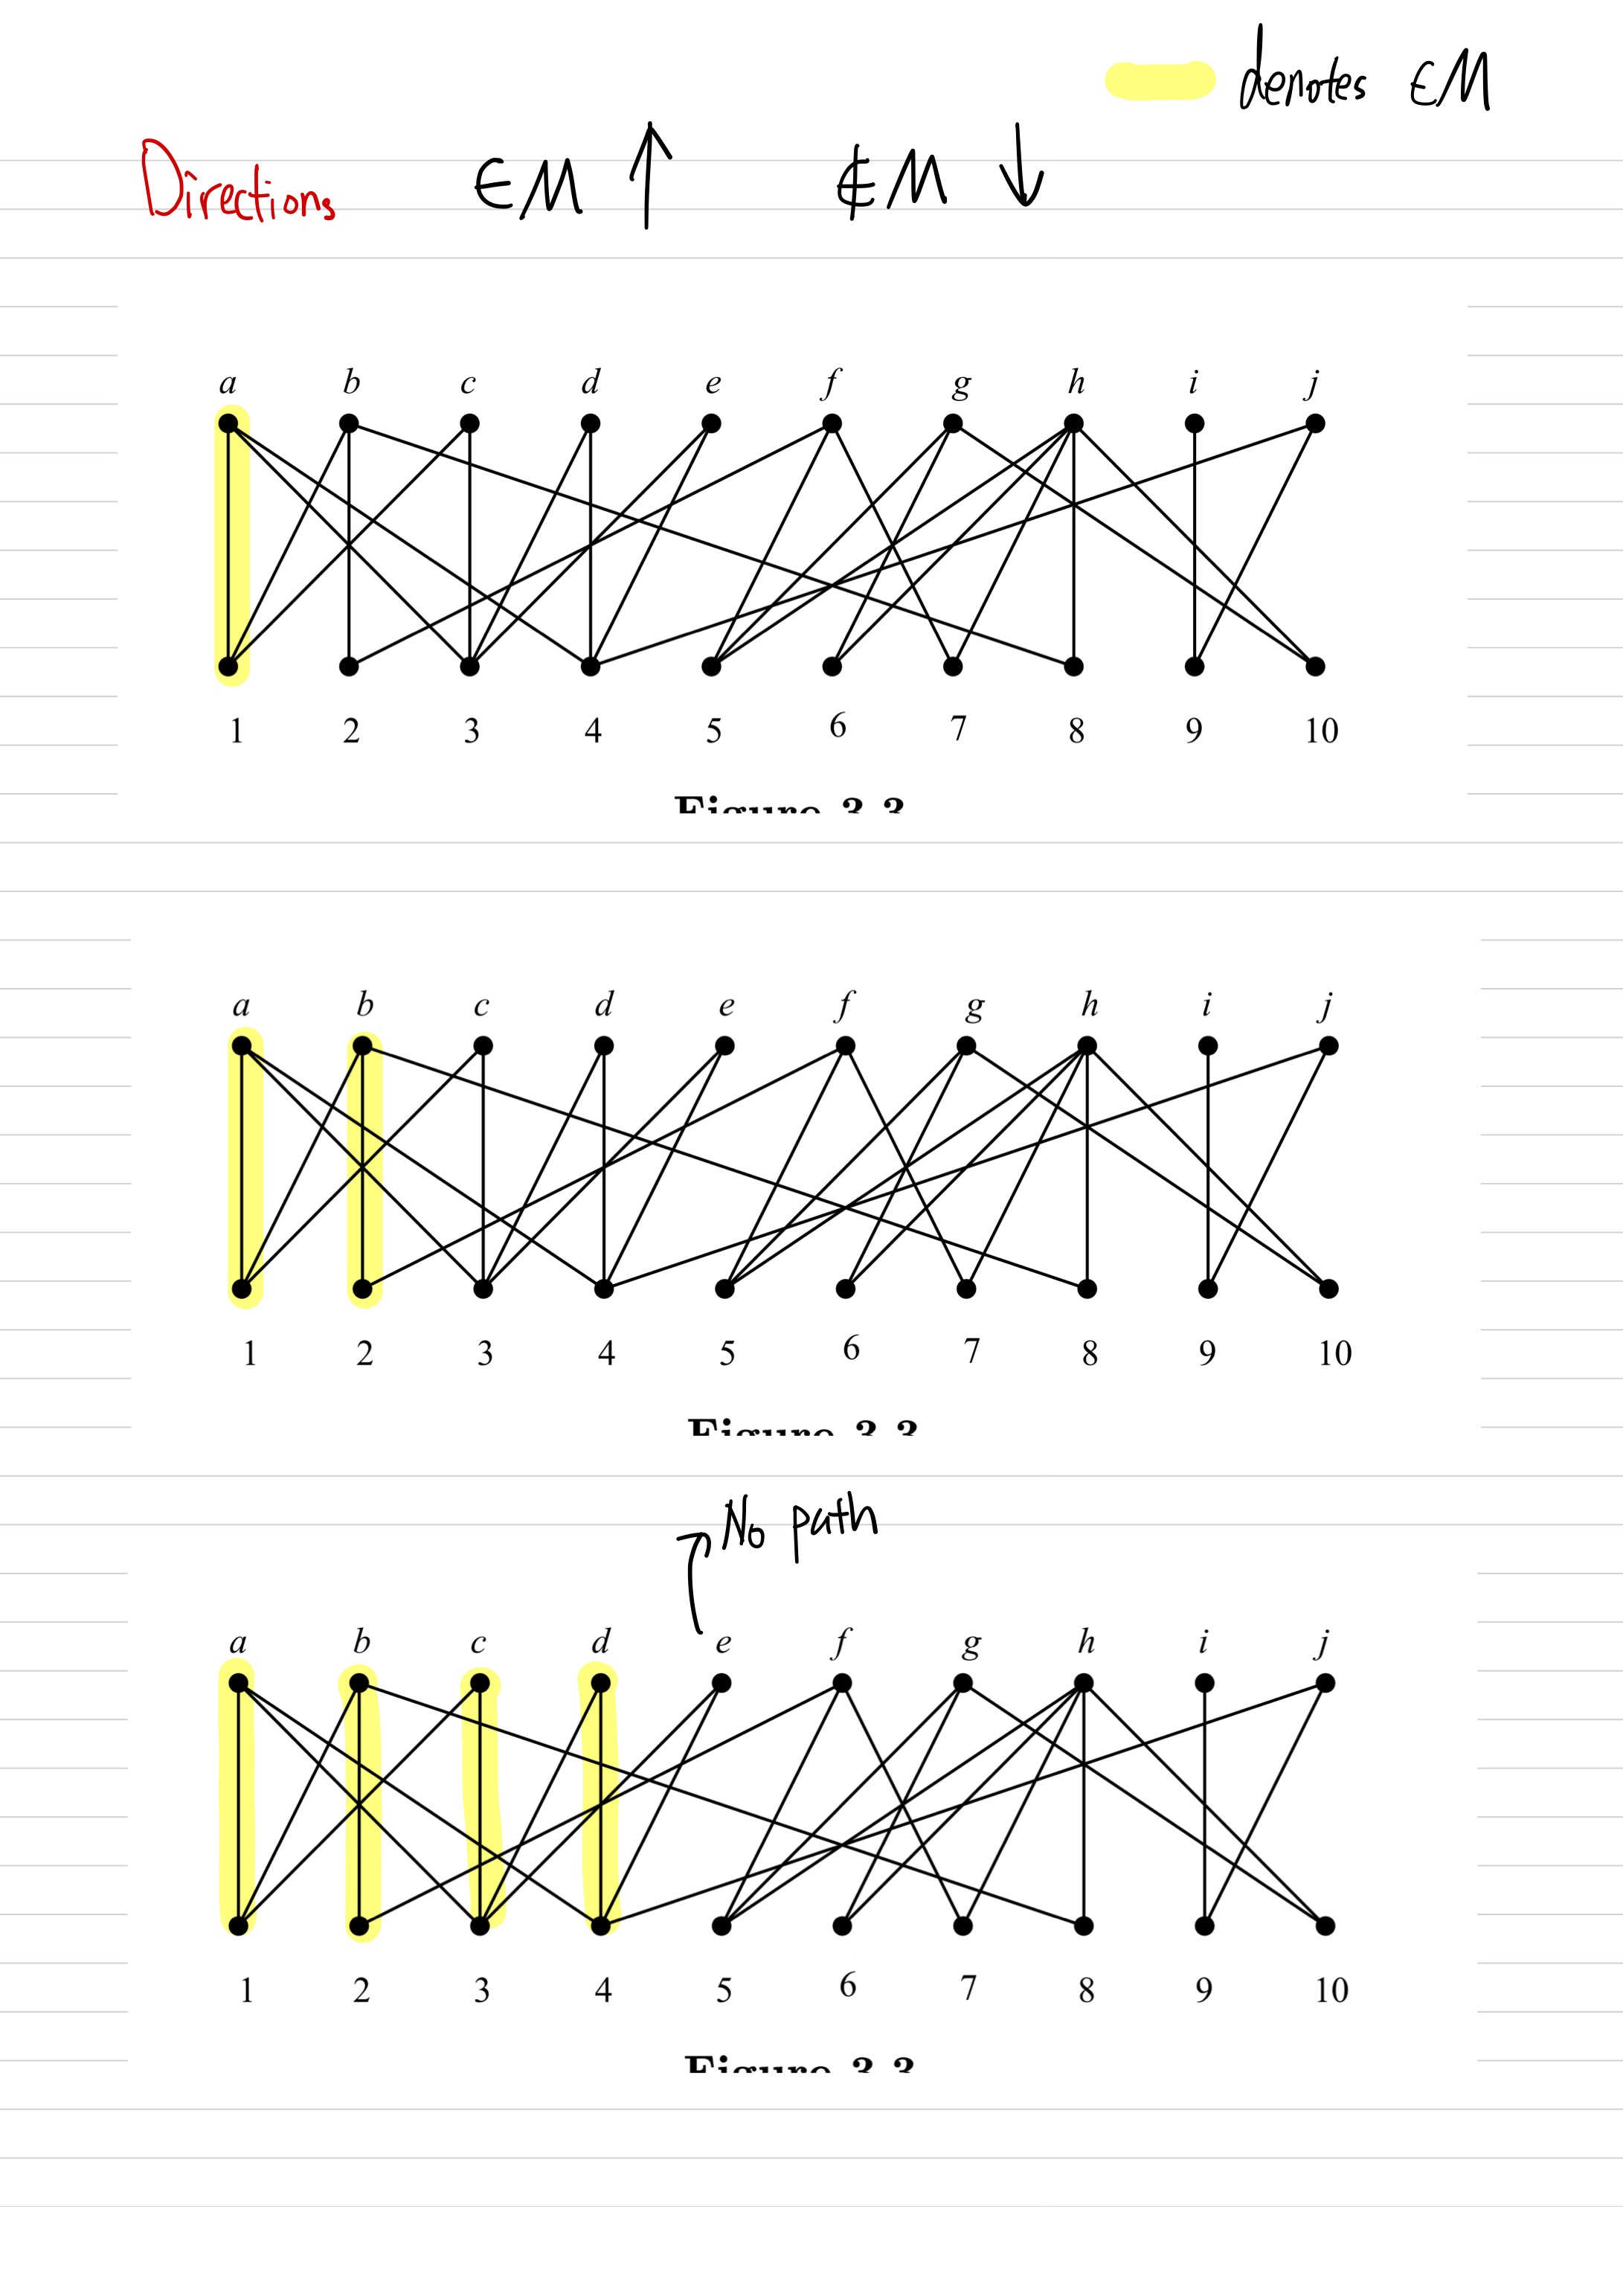
\includegraphics[width=12cm]{HW4-5.jpg}
        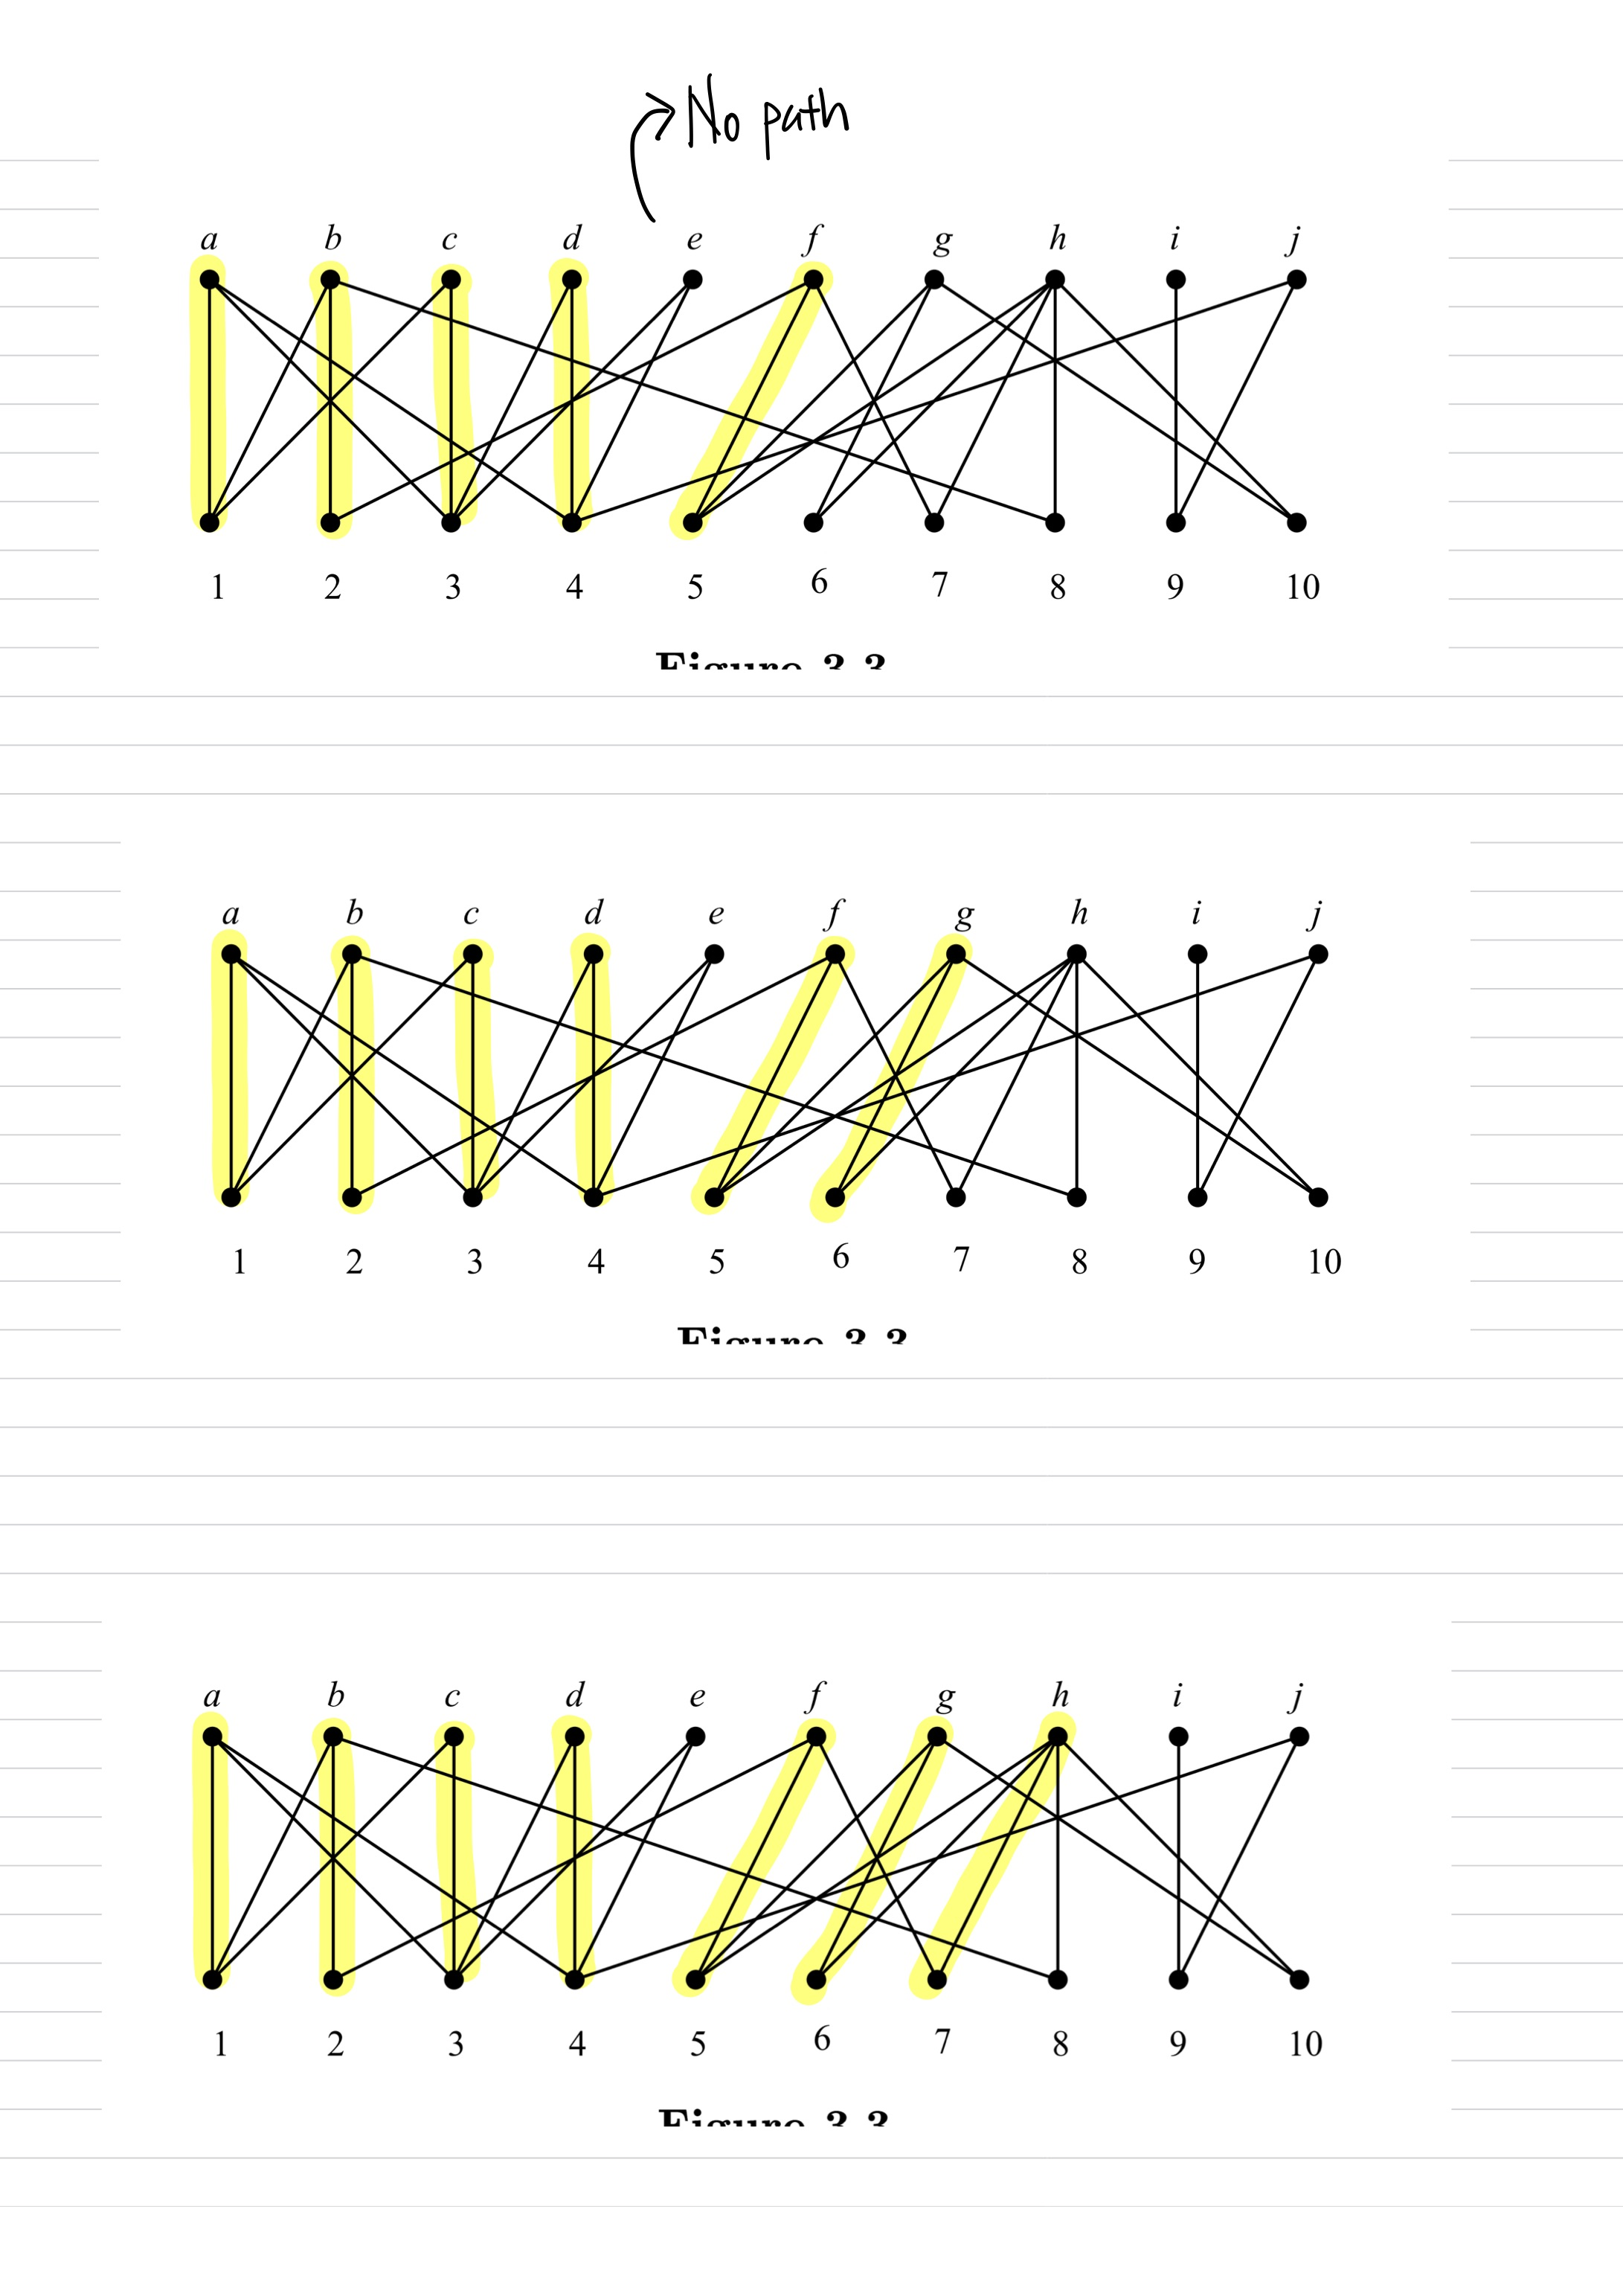
\includegraphics[width=12cm]{HW4-6.jpg}
        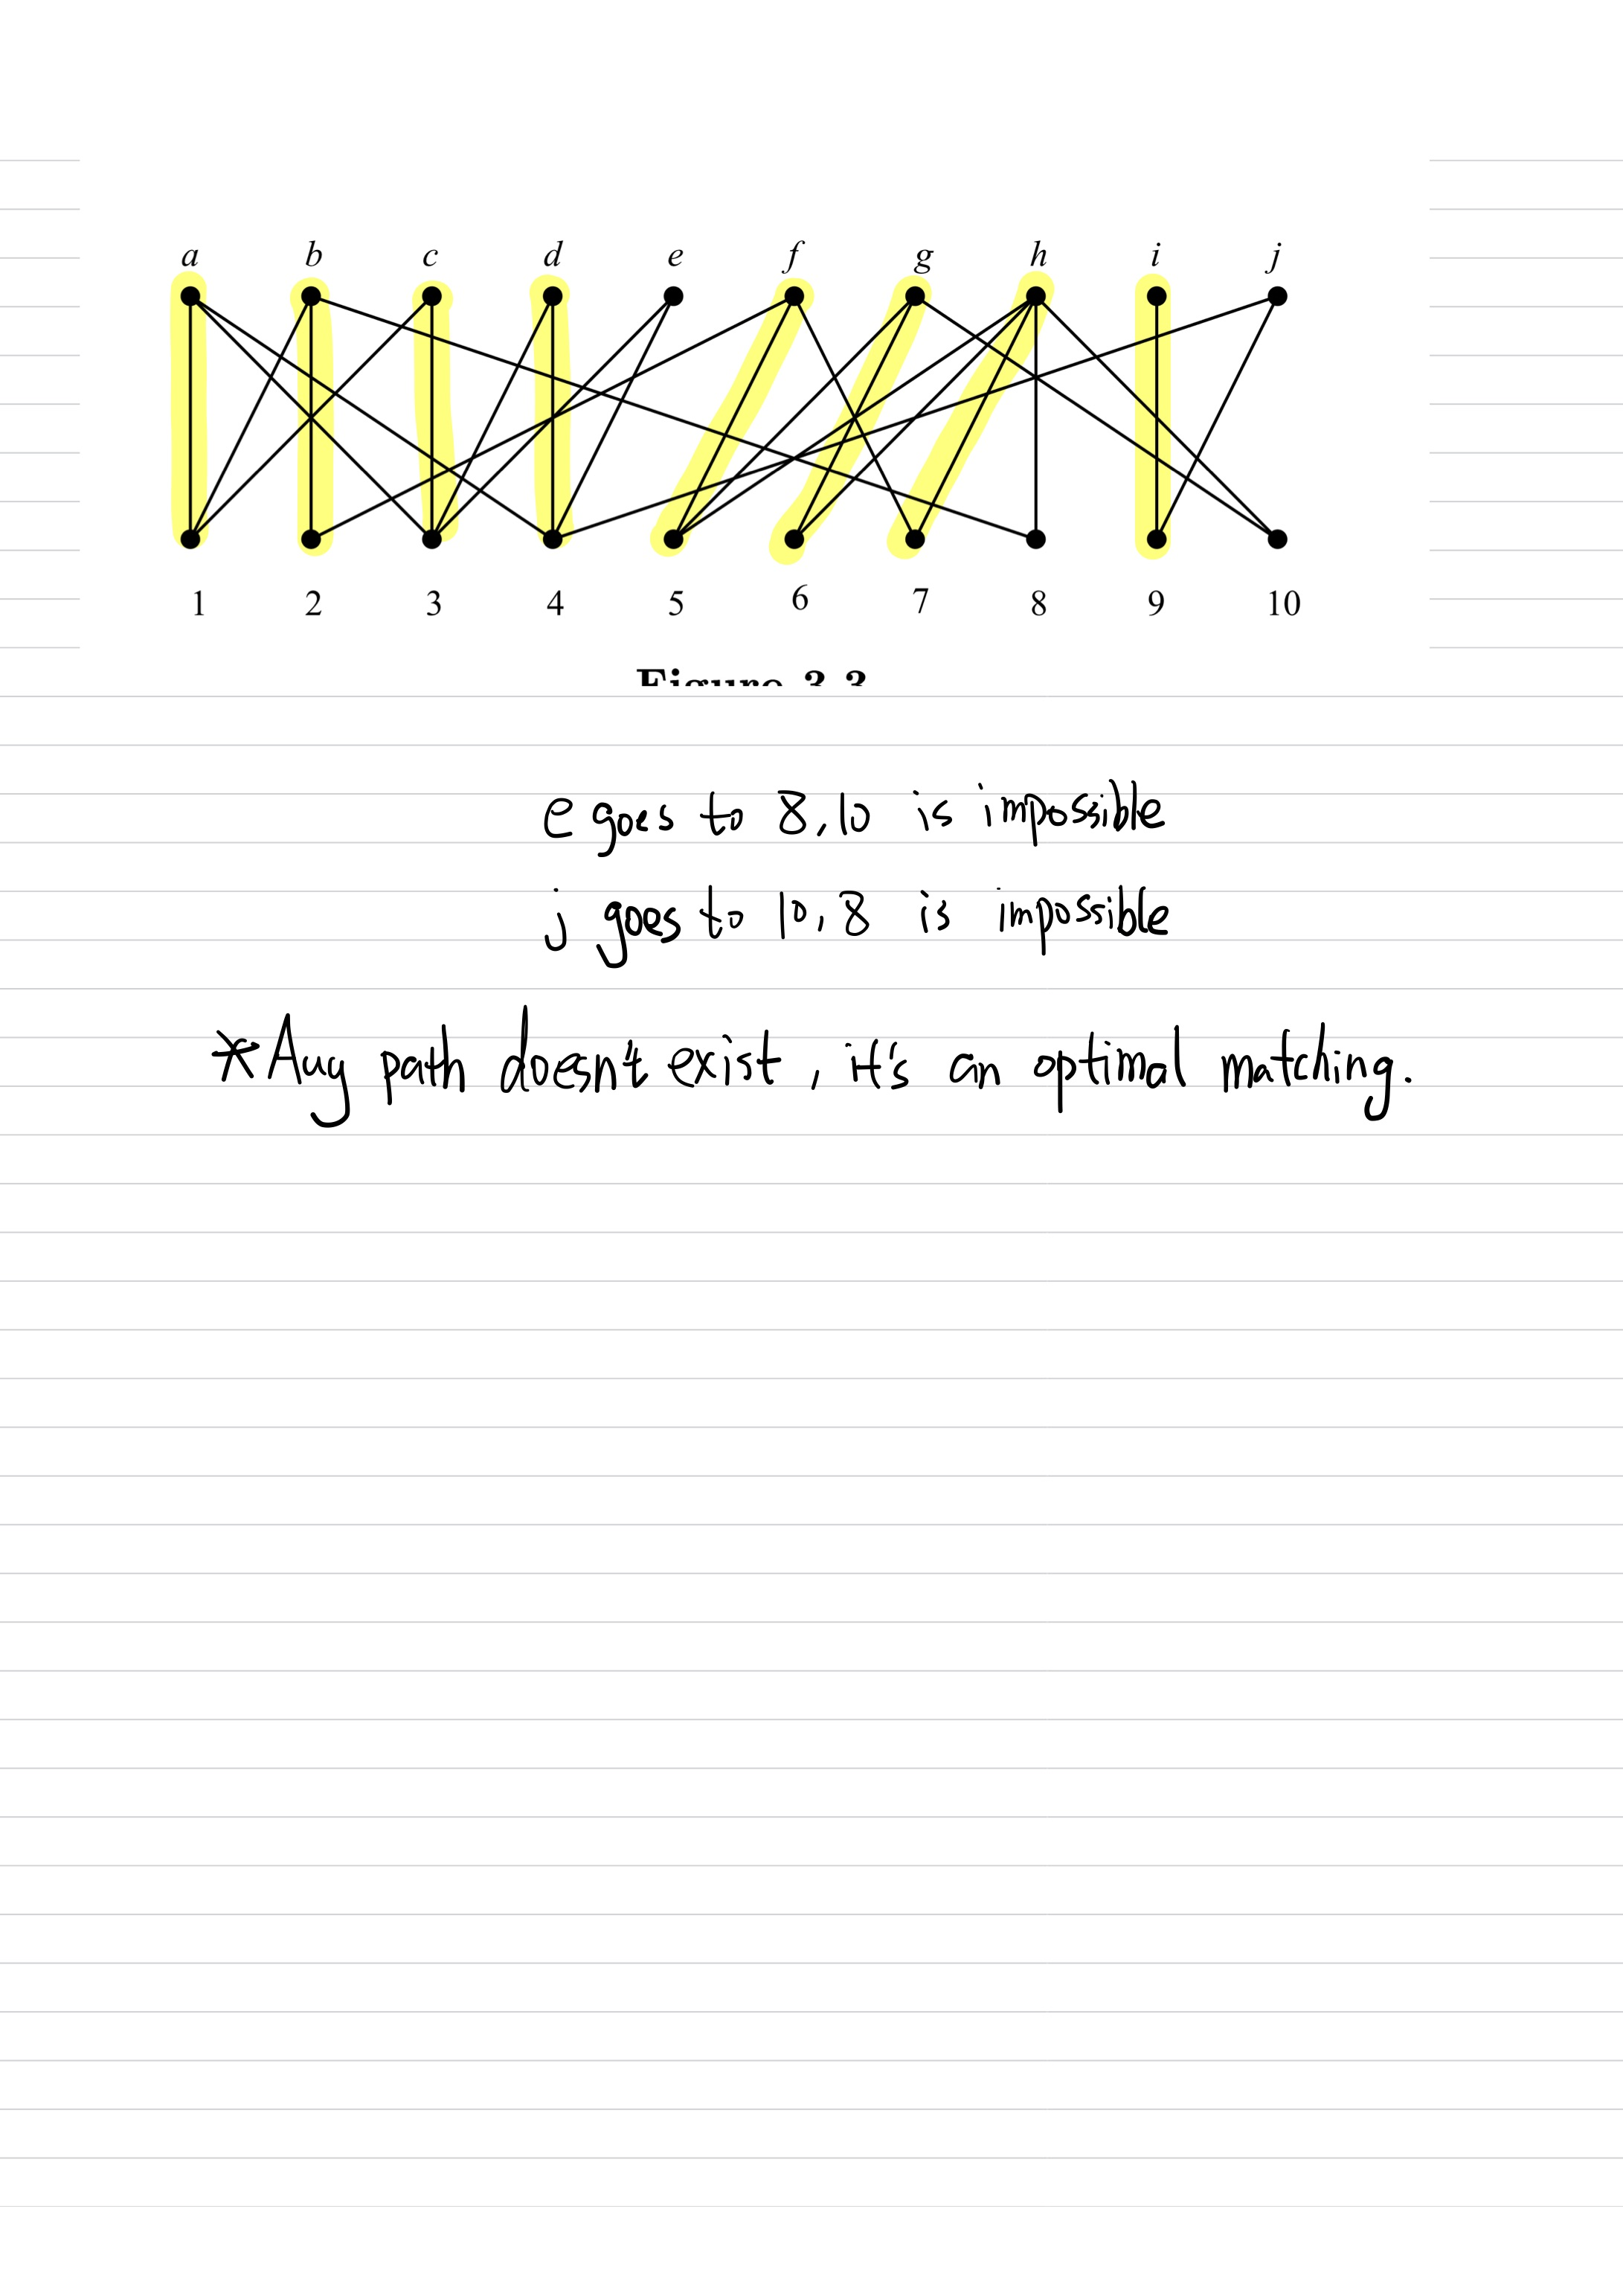
\includegraphics[width=12cm]{HW4-7.jpg}
    \end{center}
    

\end{document}